\input ../SlidePreamble
\input ../preamble

\begin{document}

{\Huge
  \centerline{\bf TTIC 31230,  Fundamentals of Deep Learning}
  \vfill
  \centerline{David McAllester, Autumn 2023}
  \vfill
\centerline{Some Information Theory}

\slide{Why Information Theory?}

The fundamental equation of deep learning involves cross-entropy.

\vfill
Cross-entropy is an information-theoretic concept.

\vfill
Information theory arises in many places and many forms in deep learning.

\slide{Entropy of a Distribution}

The entropy of a distribution $P$ is defined by

\vfill
$${\color{red} H(P) = E_{y \sim P} \left[ \;- \ln P(y)\right]}\;\;\mbox{in units of ``nats''}$$

\vfill
$${\color{red} H_2(P) = E_{y \sim P}\left[ \;- \log_2 P(y)\right]}\; \mbox{in units of bits}$$

\slide{Why Bits?}

Why is $-\log_2\;P(y)$ a number of bits?

\vfill
Example: Let $P$ be a uniform distribution on 256 values.

\vfill
$$E_{y \sim P}\;\left[\;-\log_2 P(y)\right] = - \log_2 \frac{1}{256} = \log_2 256 = 8\;\mathrm{bits} = 1\;\mathrm{byte}$$

\vfill
\centerline{\color{red} 1 nat = $\frac{1}{\ln 2}$ bits $\approx$ 1.44 bits}

\slide{Shannon's Source Coding Theorem}

Why is $-\log_2\;P(y)$ a number of bits?

\vfill
A prefix-free code for ${\cal Y}$ assigns a bit string $c(y)$ to each $y \in {\cal Y}$ such that no code string is a prefix of any other code string.

\vfill
For a probability distribution $P$ on ${\cal Y}$ we consider the average code length $E_{y \sim P}\;\left[ \;|c(y)|\right]$.

\vfill
Theorem: For any $c$ we have {\color{red} $E_{y \sim P}\;|c(y)|  \geq H_2(P)$}.

\vfill
Theorem: There exists $c$ with {\color{red} $E_{y \sim P} \;|c(y)| \leq H_2(P) +1$}.

\slide{Cross Entropy}

Let $P$ and $Q$ be two distribution on the same set.

{\color{red} $$H(P,Q) = E_{y \sim P}\;\left[ \;-\ln \;Q(y)\right]$$}

{\color{red} $$\Phi^* = \argmin_\Phi \;H(\pop,P_\Phi)$$}

\vfill
{\color{red} $H(P,Q)$} can be interpreted as the number of bits used to code draws from $P$ when using an optimal code for $Q$.

\vfill We will show
$$H(P,Q) \geq H(P)$$

\slide{KL Divergence}

Let $P$ and $Q$ be two distribution on the same set.

\vfill
\centerline{
  $\begin{array}{lrcl}
\mathrm{Entropy}: & {\color{red} H(P)} & = & {\color{red} E_{y \sim P}\;\left[-\ln\;P(y)\right]} \\
\\
\mathrm{Cross Entropy:} & {\color{red} H(P,Q)} & = & {\color{red} E_{y \sim P}\;\left[-\ln\;Q(y)\right]} \\
\\
\mathrm{KL\; Divergence:} & {\color{red} KL(P,Q)} & = & {\color{red} H(P,Q) - H(P)} \\
\\
& & = & {\color{red} E_{y \sim P}\;\;\; - \ln\;\frac{Q(y)}{P(y)}}
\end{array}$}

\vfill
We will show $KL(P,Q) \geq 0$ which implies $H(P,Q) \geq H(P)$.

\slideplain{Proving $KL(P,Q) \geq 0$: Jensen's Inequality}

\centerline{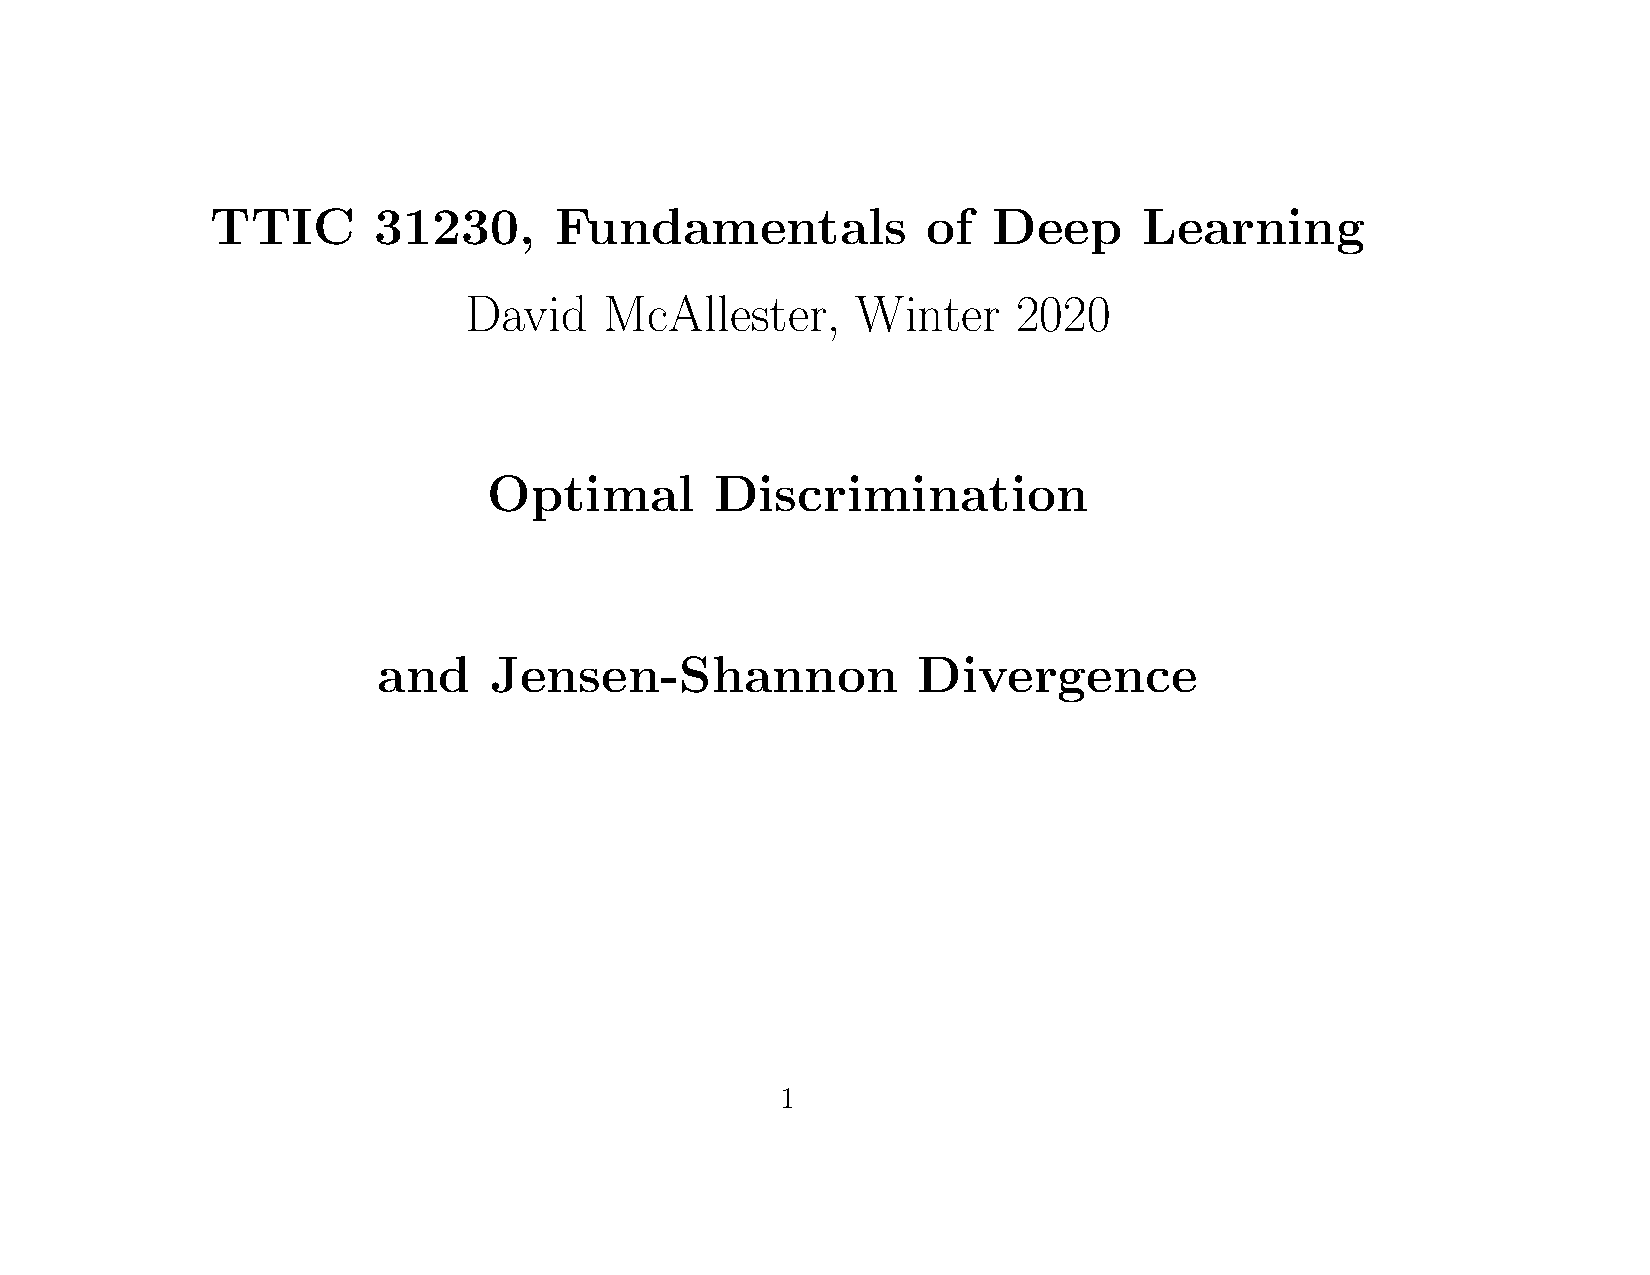
\includegraphics[height = 3.0in]{\images/Jensen}}

\vfill
For $f$ convex (upward curving) we have

\vfill
$$E[f(x)] \geq f(E[x])$$

\slide{Proving $KL(P,Q) \geq 0$}

\begin{eqnarray*}
  KL(P,Q) & = & \expectsub{y \sim P}{\left[- \ln \frac{Q(y)}{P(y)}\right]} \\
  \\
  & \geq & - \ln \expectsub{y\sim P}{\frac{Q(y)}{P(y)}} \\
  \\
  & = & - \ln \sum_y\; P(y) \frac{Q(y)}{P(y)}  \\
  \\
  & = & - \ln \sum_y Q(y) \\
  \\
  & = & 0
\end{eqnarray*}



\slide{Asymmetry of Cross Entropy}
Consider 


$$\Phi^* = \argmin_\Phi \;H(\pop,Q_\Phi)\;\;\;\;\;(1)$$

\vfill
$$\Phi^* = \argmin_\Phi \;H(Q_\Phi,\pop)\;\;\;\;\;(2)$$

\vfill
We cannot use (2) because we cannot calculate $\pop(y)$.

\vfill
For a synthetic population where $\pop(y)$ is computable (2) produces mode collapse --- $Q_\Phi$ is concentrated on the most likely value of $\pop$.

\slide{Asymmetry of KL Divergence}
Consider 


\begin{eqnarray*}
  \Phi^* & = & \argmin_\Phi \;KL(\pop,Q_\Phi) \\
  & = & \argmin_\Phi\; H(\pop,Q_\Phi)\;\;\;\;\;\;\;\;\;\;\;\;\;\;\;\;\;\;(1) \\
  \\
  \Phi^* & = & \argmin_\Phi \;KL(Q_\Phi,\pop) \\
  & = & \argmin_\Phi H(Q_\Phi,\pop) - H(Q_\Phi)\;\;\;(2)
  \end{eqnarray*}

\vfill
For a synthetic population where $\pop(y)$ is computable but $P_\Phi$ cannot perfectly model $\pop$, (2) produces mode collapse.

\slide{Conditional Entropy and Mutual Information}

Assume a joint distribution $Q$  on $x$ and $y$.

\vfill
conditional entropy:
$$H(y|x) = E_{(x,y)\sim Q}\;-\ln P(y|x)$$

\vfill
mutual information:
$$I(x,y) = H(y) - H(y|x)$$

\vfill
Suppose you dont't know anything about $x$ and $y$. The mutual information $I(x,y)$ is the expectation over a draw of $x$ of
the number of bits you learn about $y$.

\slide{Continuous Densities}

Expectations hide the discrete-continuous distinction

\vfill
$E_{x \sim P(x)}\;f(x)$ is meaningful for both discrete and continuous $P(x)$.

\vfill
$E_{x \sim P(x)}\;f(x)$ is the limit of the average of $f(x)$ over ever larger samples.

\vfill
In order to write general equations we will use capital letter notation $P(x)$ for both continuous densities and discrete distributions.

\vfill

\slide{Differential Entropy}

In the case of a continuous density (as opposed to a discrete probability) we have the notion of differential entropy.

\vfill
For a density $P(x)$ on a real value $x$ we have

\vfill
\begin{eqnarray*}
H(x) & = & E_{x \sim P(x)}\;\left[-\ln P(x)\right]
\end{eqnarray*}

\slide{Differential Cross-Entropy can Diverge to $-\infty$}

Consider the unsupervised training objective.

$$\Phi^* = \argmin_{\Phi} E_{y \sim \mathrm{train}}\;-\ln P_\Phi(y)$$

\vfill
The training set is finite (discrete).

\vfill
For each $y \in \train$ the density $P_\Phi(y)$ can go to infinity.

\vfill
This will drive the cross-entropy training loss to $-\infty$.

\slide{Differential Cross-Entropy can Diverge to $-\infty$}

$$\Phi^* = \argmin_{\Phi} E_{y \sim \mathrm{train}}\;-\ln P_\Phi(y)$$

\vfill
For a Gaussian mixture model in which some mixtures are focused on a single point
the training loss goes to $-\infty$.

\vfill
We do not want to minizing an objective that diverges to $-\infty$.

\slide{The Gaussian Noise Trick ($L_2$ Distortion)}

Assume that $\train$ is a set of pairs $(x,y)$ with $y \in R^d$.

\vfill
Linear regression invokes the Gaussian noise trick.

\vfill
Define $P_{\Phi,\sigma}(y|x)$ by
$(\hat{y}_\Phi(x) + \epsilon),\;\; \epsilon \sim {\cal N}(0,I)$.

{\huge
\begin{eqnarray*}
\Phi^* & = & \argmin_{\Phi}\;E_{(x,y)\sim \train}\left[-\ln P_{\Phi,\sigma}(y|x)\right] \\
\\
& = & \argmin_\Phi E_{(x,y)\sim \train} \left[\frac{||y - \hat{y}(x)||^2}{2\sigma^2}\right]
\end{eqnarray*}
}

$L_2$ distortion is non-negative but goes to infinity as $\sigma \rightarrow 0$.

\slide{The Gaussian Noise Trick ($L_2$ Distortion)}

For sufficiently small $\sigma$ we have that $L_2$ distortion is simply accounting for numerical precision.

\vfill
Intuitively this corresponds to using a discrete distribution defined by finite precision arithmetic with rounding error $\sigma$.

\vfill
We should {\bf not} think of the Gaussian noise trick as introducing a Bayesian assumption.

\vfill
We can prove PAC-Bayesian generalization guarantees for this trick (no Bayesian assumptions).

\slide{The Laplacian Noise Trick ($L_1$ Distortion)}

define $P_{\Phi,\lambda}(y|x)$ by $(\hat{y}_\Phi(x) + \epsilon),\;\; \epsilon \sim \softmax_\epsilon \;\lambda |\epsilon|_1$

\vfill
$$||\epsilon||_1 = \sum_i \;|\epsilon_i|$$

\vfill
{\huge
\begin{eqnarray*}
\Phi^* & = & \argmin_{\Phi}\;E_{(x,y)\sim \train}\left[-\ln P_{\Phi,\lambda}(y|x)\right] \\
\\
& = & \argmin_\Phi E_{(x,y)\sim \train} \left[\frac{||y - \hat{y}(x)||_1}{\lambda}\right]
\end{eqnarray*}
}

\slidetwo{The Gaussian Noise Trick}
{``Finite Precision'' Differential Entropy}

Define $P_\sigma(\tilde{y}|y)$ by
$$\tilde{y} = y + \epsilon,\;\epsilon \sim {\cal N}(0,I)$$

\vfill
Define $H_\sigma(y)$ by
\begin{eqnarray*}
H_\sigma(y) & = & E_{y \sim P(y),\tilde{y} \sim P_\sigma(\tilde{y}|y)}\left[ -\ln \frac{P(y)}{P(y|\tilde{y})}\right] \\
\\
& {\color{red} =} & {\color{red} I(y,\tilde{y}) \geq 0}
\end{eqnarray*}


\slidetwo{The Gaussian Noise Trick}
{``Finite Precision'' Differential Entropy}

If $P(y)$ is smooth at the scale of $\sigma$ we have $P(y|\tilde{y})$ is a Gaussian centered at $\tilde{y}$.

$$E_{y,\tilde{y}}[- \ln P(y|\tilde{y})] \approx d(\ln \sigma + \ln{\sqrt{2\pi}} + 1/2)$$

$$H_\sigma(y) \approx E_{y \sim P(y)}\left[ - \ln P(y)\right]  - d(\ln \sigma + \ln \sqrt{2\pi} + 1/2)$$

\vfill
For $P$ smooth at scale $\sigma$ this approximates mutual information and is non-negative.

\vfill
But $H_\sigma(y)$ goes to infinity (slowly) as $\sigma \rightarrow 0$.

\vfill


\slide{Summary}
      
\centerline{
  $\begin{array}{lrcl}
\mathrm{Entropy}: & {\color{red} H(P)} & = & {\color{red} E_{y \sim P}\;\left[-\ln\;P(y)\right]} \\
\\
\mathrm{Cross Entropy:} & {\color{red} H(P,Q)} & = & {\color{red} E_{y \sim P}\;\left[-\ln\;Q(y)\right]} \\
\\
\mathrm{KL\; Divergence:} & {\color{red} KL(P,Q)} & = & {\color{red} H(P,Q) - H(P)} \\
\\
\mathrm{Mutual\; Information:} & {\color{red} I(x,y)} & = & {\color{red} H(y) - H(y|x)}
\end{array}$}

\vfill
\centerline{{\color{red} $H(P,Q) \geq H(P),\;\;\;KL(P,Q) \geq 0,\;\;\;\argmin_Q\;H(P,Q) = P$}}

\slide{END}

}
\end{document}

\slide{Sensitivity to the Choice of Units}

$$H({\cal N}(0,\sigma^2)) = C + \ln \sigma$$

\vfill
Differential entropy depends on the choice of units --- a distributions on lengths will have a different entropy
when measuring in inches than when measuring in feet.

\slide{Differential KL-divergence is Meaningful}

$$KL(p,q) = \int \left( \ln \frac{P(x)}{q(x)}\right) P(x) dx$$

\vfill
Unlike differential entropy, differential KL divergence is always non-negative (but can be infinite).

\vfill
Note that $KL(P,P) = 0$ independent of $H(P)$.

\slide{Mutual Information}

$I(x,y)$ is the reduction in the number of bits we need to name $y$ as a result of observing $x$ (on average).

{\huge
\begin{eqnarray*}
I(x,y) & = & E \;\ln \frac{P(x,y)}{P(x)P(y)} \\
\\
\\
& = & E \;\ln \frac{P(x,y)}{P(x)} - \ln P(y) \\
\\
\\
& = & H(y) - H(y|x) \\
\end{eqnarray*}
}
Intuitively, how much does $x$ know about $y$?

\slide{Differential Mutual Information}

\begin{eqnarray*}
  I(x,y) & = & KL(P(x,y),P(x)P(y)) \\
  \\
  & = & E_{x,y} \ln \frac{P(x,y)}{P(x)P(y)}
\end{eqnarray*}

\vfill
Mutual information is a KL divergence and hence differential mutual information is always non-negative.

\slide{The Data Processing Inequality}

For continuous $y$ and $z$ with $z = f(y)$ we get that $H(z)$ can be either larger or smaller than $H(y)$ (consider $z = ay$ for $a >1$ vs. $a<1$).

\vfill
However, mutual information is a KL divergence and is more meaningful than entropy and for $z = f(y)$ we do have

$$I(x,z) \leq I(x,y)$$

\slide{Source Coding Theorem}

Consider a probability distribution $\mathrm{Pop}$ on a finite set $S$.

\vfill
Consider a code $C$ assigning a bit string code word $C(y_1,\ldots,y_B)$ to each possible batch of $B$ elements with $y_i \sim \mathrm{Pop}$.

\vfill
Source coding theorem: As $B \rightarrow \infty$ the optimal coding uses exactly $H(\mathrm{Pop})$
bits per batch element.

\slide{Prefix Free Codes}

Let $S$ be a finite set.

\vfill
Let $C$ be assignment of a bit string $C(y)$ to each $y \in S$.

\vfill
$C$ is called {\em prefix-free} if for $x \not = y$ we have that $C(x)$ is not a prefix of $C(y)$.

\vfill
A concatenation of sequence of prefix-free code words can be uniquely segmented (parsed) back into a sequence of code words.

\slide{Prefix-Free Codes as Trees and as Probabilities}

A prefix-free code defines a binary branching tree --- branch on the first code bit, then the second, and so on.

\vfill
The leaves of this tree are labeled with the elements of $S$.

\vfill
The code defines a probability distribution on $S$ by randomly selecting branches.

\vfill
We have $P_C(y) = 2^{-|C(y)|}$.

\slide{The Source Coding Theorem}

(1) There exists a prefix-free code $C$ such that
$$|C(y)| <= (- \log_2 \mathrm{Pop}(y)) + 1$$
and hence
$$E_{y\sim \mathrm{Pop}} |C(y)| \leq H(\mathrm{Pop}) +1$$

\vfill
(2) For any prefix-free code $C$

$$E_{y \sim \mathrm{Pop}}\;|C(y)| = E_{y \sim \pop} -\ln \;P_C(y) = H(\pop,P_C) \geq H(\mathrm{Pop})$$

\slide{Code Construction}

\vfill
We construct a code by iterating over $y \in S$ in order of decreasing probability (most likely first).

\vfill
For each $y$ select a code word $C(y)$ (a tree leaf) with length (depth)

\vfill
$$|C(y)| = \lceil - \log_2 \mathrm{Pop}(y)\rceil$$

\vfill
and where $C(y)$ is not an extension of (under) any previously selected code word.

\slide{Code Existence Proof}

At any point before coding all elements of $S$ we have
$$\sum_{y \in \mathrm{Defined}} 2^{-|C(y)|} \leq \sum_{y \in \mathrm{Defined}} \mathrm{Pop}(y) < 1$$

\vfill
Therefore there exists an infinite descent into the tree that misses all previous code words.

\vfill
Hence there exists a code word $C(x)$ not under any previous code word with
$|C(x)| = \lceil - \log_2 \mathrm{Pop}(y)\rceil$.

\vfill
Furthermore $C(x)$ is at least as long as all previous code words and hence $C(x)$ is not a prefix of any previously selected code word.

\slidetwo{Huffman Coding Produces an Optimal Code}
{For Finite Distributions}

Maintain a list of trees $T_1,\;\dots,\;T_N$ where each leaf of each tree is labeled with a population element $y$.

\vfill
We will write $y \in T_i$ to mean that some leaf of $T_i$ is labeled with $y$ and for $y \in T_i$ write $d(y,T_i)$ for the depth
of the leaf labeled with $y$ in the tree $T_i$.

\vfill
Initially each tree is just one root node labeled with a single $y$ value and every $y$ value labels some tree.

\slide{Tree Weight}

\vfill
We define the weight of a free $T_i$ to be the total probability mass of the the items labeling the leaves.

$$W(T_i) = \sum_{y \in T_i}\;\pop(y)$$

\vfill
The Huffman coding algorithm repeatedly merges the two trees of lowest weight into a single tree until all trees are merged.

\vfill
When all trees are merged the weight of the final tree is the expected code length.

\slide{Optimality of Huffman Coding}

{\bf Theorem}: The Huffman code $T$ for $\mathrm{Pop}$ gives an optimal code $C$ --- for any other tree $T'$ defining code $C'$ we have

$$E_{y \sim \pop}\;|C(y)| \leq E_{y \sim \pop} |C'(y)|$$

\vfill
{\bf Invariant:} The merge operation preserves the invariant that there exists an optimal tree including
all the subtrees on the list.

\slide{The Merge Operation Preserves the Invariant}

Assume there exists an optimal tree containing the given subtrees.

\vfill
Consider the two subtrees $T_i$ and $T_j$ of minimal weight.  Without loss of generality we can assume that $T_i$ is at least as deep as $T_j$.

\vfill
Swapping the sibling of $T_i$ for $T_j$ brings $T_i$ and $T_j$ together.  This can only improve the average depth (next slide).

\slide{Why The Swap Can Only Improve the Tree}

We can swap a heavier deeper tree for a shallower lighter tree.

\vfill
For a subtree $T_i$ of an optimal tree $T$ let $d(T_i)$ be the depth of $T_i$ in $T$.

Swapping $T_1$ and $T_2$ replaces a cost of $d(T_i)W(T_i) + d(T_2)W(T_2)$ with $d(T_1)W(T_2) + d(T_2)W(T_1)$.

\vfill
For $d(T_1) \geq d(T_2)$ and $W(T_1) \geq W(T_2)$ we have

\vfill
$$d(T_1)W(T_1) + d(T_2)W(T_2) \geq d(T_1)W(T_2) + d(T_2)W(T_1)$$


\slide{END}

\end{document}
